% This is the Reed College LaTeX thesis template. Most of the work 
% for the document class was done by Sam Noble (SN), as well as this
% template. Later comments etc. by Ben Salzberg (BTS). Additional
% restructuring and APA support by Jess Youngberg (JY).
% Your comments and suggestions are more than welcome; please email
% them to cus@reed.edu
%
% See http://web.reed.edu/cis/help/latex.html for help. There are a 
% great bunch of help pages there, with notes on
% getting started, bibtex, etc. Go there and read it if you're not
% already familiar with LaTeX.
%
% Any line that starts with a percent symbol is a comment. 
% They won't show up in the document, and are useful for notes 
% to yourself and explaining commands. 
% Commenting also removes a line from the document; 
% very handy for troubleshooting problems. -BTS

% As far as I know, this follows the requirements laid out in 
% the 2002-2003 Senior Handbook. Ask a librarian to check the 
% document before binding. -SN

%%
%% Preamble
%%
% \documentclass{<something>} must begin each LaTeX document
\documentclass[12pt,twoside]{reedthesis}
% Packages are extensions to the basic LaTeX functions. Whatever you
% want to typeset, there is probably a package out there for it.
% Chemistry (chemtex), screenplays, you name it.
% Check out CTAN to see: http://www.ctan.org/
%%
\usepackage{graphicx,latexsym} 
\usepackage{amssymb,amsthm,amsmath}
\usepackage{longtable,booktabs,setspace} 
\usepackage{chemarr} %% Useful for one reaction arrow, useless if you're not a chem major
\usepackage[hyphens]{url}
\usepackage{rotating}
\usepackage{natbib}
\usepackage{amsthm}
\usepackage[english]{babel}
\usepackage{float}
\usepackage{graphicx}
\usepackage{amssymb}
\usepackage{hyperref}
\usepackage[utf8]{inputenc}
\usepackage{listings}
\usepackage{pgf, tikz}
\usepackage{xcolor}
\usepackage{geometry}
\usepackage [english]{babel}
\usepackage [autostyle, english = american]{csquotes}
\MakeOuterQuote{"}
\geometry{margin=1in}
\usepackage[utf8]{inputenc}
\newtheorem{theorem}{Theorem}
\newtheorem{example}{Example}
\newtheorem{remark}{Remark}[section]
\newtheorem{definition}{Definition}[section]
\theoremstyle{definition}
\newcommand{\dsep}{\perp \!\!\!\perp}
% Comment out the natbib line above and uncomment the following two lines to use the new 
% biblatex-chicago style, for Chicago A. Also make some changes at the end where the 
% bibliography is included. 
%\usepackage{biblatex-chicago}
%\bibliography{thesis}

% \usepackage{times} % other fonts are available like times, bookman, charter, palatino

\title{My Final College Paper}
\author{Your R. Name}
% The month and year that you submit your FINAL draft TO THE LIBRARY (May or December)
\date{May 200x}
\division{Mathematics and Natural Sciences}
\advisor{Advisor F. Name}
%If you have two advisors for some reason, you can use the following
%\altadvisor{Your Other Advisor}
%%% Remember to use the correct department!
\department{Mathematics}
% if you're writing a thesis in an interdisciplinary major,
% uncomment the line below and change the text as appropriate.
% check the Senior Handbook if unsure.
%\thedivisionof{The Established Interdisciplinary Committee for}
% if you want the approval page to say "Approved for the Committee",
% uncomment the next line
%\approvedforthe{Committee}

\setlength{\parskip}{0pt}
%%
%% End Preamble
%%
%% The fun begins:
\begin{document}

  \maketitle
  \frontmatter % this stuff will be roman-numbered
  \pagestyle{empty} % this removes page numbers from the frontmatter

% Acknowledgements (Acceptable American spelling) are optional
% So are Acknowledgments (proper English spelling)
    \chapter*{Acknowledgements}
	I want to thank a few people.

% The preface is optional
% To remove it, comment it out or delete it.
    \chapter*{Preface}
	This is an example of a thesis setup to use the reed thesis document class.
	
	

    \chapter*{List of Abbreviations}

	

    \tableofcontents
% if you want a list of tables, optional
    \listoftables
% if you want a list of figures, also optional
    \listoffigures

% The abstract is not required if you're writing a creative thesis (but aren't they all?)
% If your abstract is longer than a page, there may be a formatting issue.
    \chapter*{Abstract}
	The preface pretty much says it all.
	
	\chapter*{Dedication}
	You can have a dedication here if you wish.

  \mainmatter % here the regular arabic numbering starts
  \pagestyle{fancyplain} % turns page numbering back on

%The \introduction command is provided as a convenience.
%if you want special chapter formatting, you'll probably want to avoid using it altogether

    \chapter*{Introduction}
         
	\chaptermark{Introduction}
	\markboth{Introduction}{Introduction}
	% The three lines above are to make sure that the headers are right, that the intro gets included in the table of contents, and that it doesn't get numbered 1 so that chapter one is 1.

% Double spacing: if you want to double space, or one and a half 
% space, uncomment one of the following lines. You can go back to 
% single spacing with the \singlespacing command.
% \onehalfspacing
% \doublespacing
	
	
    \chapter{The First}

\section{Background: Graphs, D-separation, Causality}
The idea of cause and effect has been studied and discussed in philosophy for centuries, but  the formalization of causality in mathematics, statistics, and computer science is much more recent. One framework in particular, Judea Pearl's Structural Causal Models (SCMs),  [ref Pearl 1996] is flexible, widely used, and mathematically elegant. However, before we can give SCMs a serious treatment, it is helpful to introduce definitions for the graphical machinery that most analysis of SCMs rely on.

\subsection{Directed Acylic Graphs}
\theoremstyle{definition}
\begin{definition}
A $\mathbf{graph}$ $G$ is a pair $G = (V, E)$ where $V$ denotes a set of nodes (sometimes called vertices) and $E \subseteq \{(i,j) | i,j \in V\}$ denotes a set of edges between nodes.
\end{definition}
Conventions differ, but for our purposes, an edge $(i,j) \in E$ is considered to be a \textbf{edge},  read as "an edge from node $i$ to node $j$".  For easy reading, we write $i \rightarrow j$ whenever $(i,j) \in E$. In the figures that frequently accompany graphs, an edge $(i,j)$ is depicted as an arrow from node $i$ to node $j$.

\begin{figure}
\centering
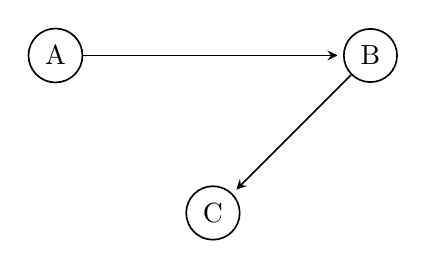
\begin{tikzpicture}[
            > = stealth, % arrow head style
            shorten > = 2pt, % don't touch arrow head to node
            auto,
            node distance = 3cm, % distance between nodes
            semithick % line style
        ]
\node[shape=circle,draw=black] (A) at (0,0) {A};
\node[shape=circle,draw=black] (B) at (4,0) {B};
\node[shape=circle,draw=black] (C) at (2,-2) {C};

 \path [->] (A) edge node[left] {} (B);
 \path [->] (B) edge node[left] {} (C);


\end{tikzpicture}
\caption{Graphs corresponding to $V = \{A,B,C\}$, $E = \{(A,B), (B,C)\}$ } \label{fig:M1}
\end{figure}

 Often times we are interested in how different nodes in a particular graph are or are not connected to one another. In this spirit we define paths.
 
\begin{definition}
A $\mathbf{path}$ $p$ between nodes $v_1, v_n \in V$ is a sequence $v_1, v_2, ..., v_n \in V$  of distinct nodes such that either $(v_i, v_{i+1}) \in E$ or $(v_i, v_{i+1}) \in E$ edge always exists between $v_i$ and $v_{i+1}$. When $v_i \rightarrow v_{i+1}$ ($(i, i-1) \in E$) for all $i \in \{1,2,...,n \}$, we say $p$ is a $\mathbf{directed \ path}$.
\end{definition}




For a directed graph $G$ and a particular node $v \in V$, we define several sets of related nodes. The \textbf{parents} of $v$, denoted $PA_v$, are the nodes with a directed edge ending at $v$, $\{j \in V | j \rightarrow v \}$ and similarly the \textbf{children}, denoted $CH_v$, of $v$ are those nodes which $v$ has a directed edge to, $\{j \in V | v \rightarrow j \}$. 

Extending these definitions, we define the \textbf{ancestors} of $v$, $AN_v$, as all the nodes from which a directed path to $v$ exists,  $\{j \in V | j \rightarrow ... \rightarrow v \}$. Likewise we define \textbf{descendants} $DE_v$ of $v$ as the nodes for which a directed path from $v$ exists,   $\{j \in V | v \rightarrow ... \rightarrow j\}$ [ref Peters chp 6.1]. With these in place, we progress to the next definition.

\begin{definition}
A directed graph $G = (V,E)$ is said to be an \emph{\textbf{directed acyclic graph}} (DAG) if for all nodes $v \in V$, $DE_v \cap AN_v = \emptyset$. That is, a directed graph is a DAG when there is never a directed path from a node to itself. 
\end{definition}

\begin{figure}
\centering
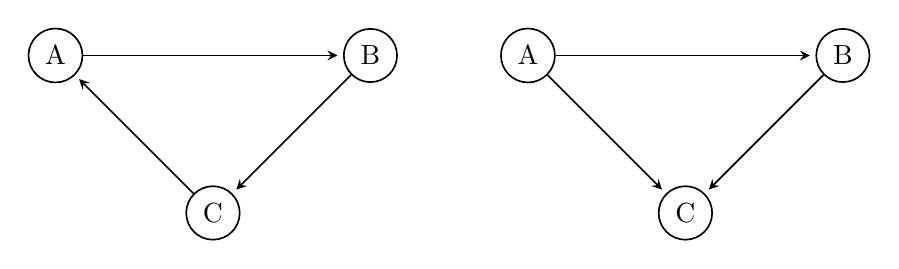
\begin{tikzpicture}[
            > = stealth, % arrow head style
            shorten > = 2pt, % don't touch arrow head to node
            auto,
            node distance = 3cm, % distance between nodes
            semithick % line style
        ]
\node[shape=circle,draw=black] (A) at (0,0) {A};
\node[shape=circle,draw=black] (B) at (4,0) {B};
\node[shape=circle,draw=black] (C) at (2,-2) {C};

 \path [->] (A) edge node[left] {} (B);
 \path [->] (B) edge node[left] {} (C);
  \path [->] (C) edge node[left] {} (A);


\node[shape=circle,draw=black] (A) at (6,0) {A};
\node[shape=circle,draw=black] (B) at (10,0) {B};
\node[shape=circle,draw=black] (C) at (8,-2) {C};

\path [->] (A) edge node[left] {} (B);
\path [->] (B) edge node[left] {} (C);
\path [->] (A) edge node[left] {} (C);
\end{tikzpicture}

\caption{Cyclic (left) and acyclic (right) graphs on the nodes $A,B,C$} \label{fig:M1}
\end{figure}

Now that we have defined DAGs, we can advance to a relevant application, Bayesian networks.

\subsection{Bayesian Networks}

Before we do so, we review some basic definitions from probability.

\begin{definition}
For random variables $X_1, X_2, ..., X_n$, the \textbf{joint distribution} with associated joint probability function $P(x_1, x_2, ..., x_n)$ gives the probability of every possible combination of values for $X_1, X_2, ..., X_n$. For any subset $\{Y_1,...,Y_k\} \subseteq \{X_1, X_2, ..., X_n\}$, the probability distribution for $Y_1, Y_2, ..., Y_k$, is called the \textbf{marginal distribution}. Finally, for a subset 
\end{definition}



\subsection{D-Separation}
Graphical structure can allow us to reason about causal and statistical relationships. One of the essential tools is d-separation. To develop the intuition, consider the very basic DAG $A \rightarrow B \rightarrow C$. There is exactly one directed path from $A$ to $C$, and the path passes through $B$. So to get to $C$ from $A$ you need to pass through $B$. In this way, we say that $B$ blocks the directed path from $A$ to $C$. We extend this notion [ref Pearl 2008], [ref Peters 2017].

\begin{definition}
Given a directed graph $G$, a path $p$ from node $v_1$ to node $v_n$ is said to be \textbf{\emph{blocked}} by a set $S$ (with $S \cap \{v_1, v_n\} = \emptyset$) if:
\begin{enumerate}
\item $v_j \in S$ and $p$ contains a $\mathbf{chain}$: $v_{j-1} \rightarrow v_j \rightarrow v_{j+1}$ or $v_{j-1} \leftarrow v_j \leftarrow v_{j+1}$, or

\item $v_j \in S$ and $p$ contains a \textbf{\emph{fork}}: $v_{j-1} \leftarrow v_j \rightarrow v_{j+1}$, or

\item $v_j \notin S$ and $DE_{v_j} \cap S = \emptyset$ and $p$ contains a \textbf{\emph{collider}}: $v_{j-1} \rightarrow v_j \leftarrow v_{j+1}$. As we will see, colliders play an especially important role in the analysis of causal DAGs.
\end{enumerate}
\end{definition}

\begin{example}
Consider a path $A \rightarrow B \rightarrow C \leftarrow D \rightarrow E$ between nodes $A$ and $E$. There are many sets that block this path. For one, there is a collider on the path. This means that any set which does not include $C$ or any elements of $DE_C$ would successfully block the path. However, we could also pick $S = \{B\}$, $S= \{D\}$, or $S = \{B,D\}$ as blocking sets since the path contains a chain at $B$ and a  fork at $D$. Importantly, if we have either of these nodes in our blocking set, we could include $C$ as well because the first blocking condition would be satisfied, even though the second would not. In fact, the only $S \subseteq \{B,C,D\}$ that would not block the path is $S = \{C\}$.
\end{example}

With blocking defined, we address d-separation. 

\begin{definition}
For a DAG $G$, two sets of nodes $A,B \in G$ are said to be  \textbf{\emph{d-separated}} by a set $S$ if all paths between $A$ and $B$ are blocked by $S$. We denote d-separation by the symbol $\perp \!\!\!\perp_G$, with the statement "In DAG $G$, $A$ is d-separated from $B$ by $S$" expressed as $A \dsep_G B | S$. 
\end{definition}

\begin{remark}
If $A \dsep_G B | S$ then $B \dsep_G A | S$
\end{remark}
\begin{example}
Consider the DAG $G$ below.

    $$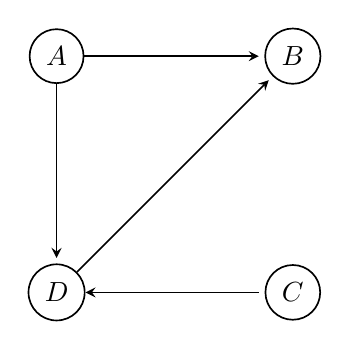
\begin{tikzpicture}[
            > = stealth, % arrow head style
            shorten > = 2pt, % don't touch arrow head to node
            auto,
            node distance = 3cm, % distance between nodes
            semithick % line style
        ]
        

        \tikzstyle{every state}=[
            draw = black,
            thick,
            fill = white,
            minimum size = 4mm
        ]

        \node[shape=circle,draw=black] (A) {$A$};
        \node[shape=circle,draw=black] (B) [right of=A] {$B$};
        \node[shape=circle,draw=black] (C) [below of=B] {$C$};
        \node[shape=circle,draw=black] (D) [left of=C] {$D$};

        \path[->] (A) edge node {} (B);
	    \path[->] (A) edge node {} (D);
	    \path[->] (D) edge node {} (B);
	    \path[<-] (D) edge node {} (C);
    \end{tikzpicture}$$
\end{example}

Which nodes can be d-separated, and by which blocking sets? Nodes which are connected by an edge cannot be d-separated. To see why, take $A$ and $B$. Although some paths between $A$ and $B$ can be blocked, the path $A \rightarrow B$ contains no nodes other than $A$ and $B$ and therefore cannot be blocked. Since there is no set that can block the path, $A$ and $B$ are not able to be d-separated. So consider $A$ and $C$, two nodes which are not connected by an edge. There are two paths between $A$ and $C$, $A \rightarrow B \leftarrow D \leftarrow C$ and $A \rightarrow D \leftarrow C$. Both of these paths include a collider. Of the four possible blocking sets, $\emptyset, \{B\}, \{D\}, \{B,D\}$, all but $\emptyset$ include a collider node for paths that are not blocked by other means. Then $A \dsep_G C | \emptyset$ and no other sets will work. What about $B$ and $C$? Again there are two paths: $B \leftarrow D \leftarrow C$ and $B \leftarrow A \rightarrow D \leftarrow C$. The second path contains a collider, and therefore is blocked by $\emptyset$, but the first path cannot be. To block $B \leftarrow D \leftarrow C$ we must have $D$ in our blocking set. So, $B \dsep_G C | D$, but we can also include $A$ since doing so will not unblock a path with a collider. Then $B \dsep_G C | D,A$.


\subsection{Structural Causal Models}
Many questions in the natural and social sciences involve understanding the way that one set of factors (e.g. genes, medicines, social policies) influence others (e.g. disease risk, mortality, childhood poverty rates). In these cases, the language and  of classical statistics is often inadequate. The tools of hypothesis testing, (linear) regression, interval estimation, etc. can tell us much about relationships in the data, but except in the highly constrained setting of randomized controlled trials, very little about cause and effect. These limitations are not just theoretical. Many longstanding controversies and debates within the sciences come down to disagreements over which factors associated with a particular outcome are causing the outcome. 

A paradigmatic example of such a controversy is over the relationship between cigarette smoking and lung cancer. Today, it is uncontroversial that smoking cigarettes (especially habitually over a long period of time) increases a person's risk of contracting lung cancer. This is a causal relationship, and we might express our belief in this relationship as a \textbf{\emph{causal model}} in which a person's risk of contracting lung cancer is a \emph{function} of a person's smoking habits (for simplicity, we  pretend that smoking is the only such causal factor).

So, let $L$ be a random variable denoting whether or not a person contracts lung cancer and $S$ be a random variable denoting smoking. Under our causal model in which smoking is the only structural cause of lung cancer, we express $L$ as a function of $S$:

$$L :=f(S, N_L),$$
$$S := N_S.$$ 

Here, the use of $:=$ denotes an assignment rather that an algebraic relationship [ref Peters] and $N_L$ is a noise term capturing random effects on lung cancer risk, and $N_S$ a noise variable for cigarette smoking. Together, these two assignments are a  structural causal model.  Now that we have an SCM, we can express the structure as a DAG. Since $L$ is assigned as a function of smoking but $S$ is not caused by any factors in our model, we would express our model as a directed edge going from $S$ to L:



$$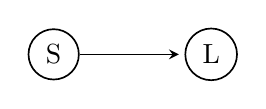
\begin{tikzpicture}[
            > = stealth, % arrow head style
            shorten > = 2pt, % don't touch arrow head to node
            auto,
            node distance = 3cm, % distance between nodes
            semithick % line style
        ]
\node[shape=circle,draw=black] (S) at (8,0) {S};
\node[shape=circle,draw=black] (L) at (10,0) {L};


 \path [->] (S) edge node[left] {} (L);



\end{tikzpicture}$$

However, historically, this causal structure was not the only one suggested to explain the association between lung cancer and smoking. One particularly illustrious detractor of this theory was British statistician R. A. Fisher, a foundational figure in modern statistics (and a heavy smoker) [ref Fisher]. In Fisher's view, there was no causal effect of smoking on lung cancer, rather, an underlying genetic factor was responsible for both a predisposition to smoking and a higher risk of developing lung cancer. So Fisher's causal model would have looked like:
$$L :=f(G, N_L),$$
$$S := f(G, N_S),$$
$$G := N_G.$$ 
Where $G$ is the genetic factor. As before, the structure of this model can be expressed as a graph:

$$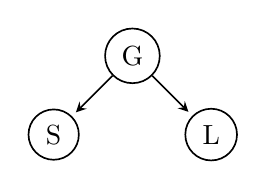
\begin{tikzpicture}[
            > = stealth, % arrow head style
            shorten > = 2pt, % don't touch arrow head to node
            auto,
            node distance = 3cm, % distance between nodes
            semithick % line style
        ]
\node[shape=circle,draw=black] (G) at (9,1) {G};
\node[shape=circle,draw=black] (S) at (8,0) {S};
\node[shape=circle,draw=black] (L) at (10,0) {L};

 \path [->] (G) edge node[left] {} (L);
 \path [->] (G) edge node[left] {} (S);
\end{tikzpicture}$$


In this way, every SCM entails a directed graph. Although it is entirely possible for an SCM to entail a graph that has cycles, we focus our attention on the case where the graph entailed is a DAG. Importantly, these two (graphical) models imply different observational joint distributions. Without having specified the functions, little can be said about the joint distribution entailed by the model, however, one important property is built in to every SCM.

\begin{definition}[Markov property]
In any SCM $C$ with entailed graph $G$, if $A \dsep_G B | S \implies A \dsep B | S$ for all disjoint sets of nodes $A,B,S$. That is, every d-separation in the graph corresponds to a conditional independence in the joint distribution. This fact is implied by the definition of SCMs and is called the \emph{\textbf{Markov Property}}.
\end{definition}

[This seems important enough to reproduce a proof but I will have to spend a little more time than I have tonight]

This result is a powerful tool that allows us to test how well differing causal models comport with the observational data.  Returning to Fisher's suggestion that an underlying genetic cause was responsible for the association of smoking with lung cancer, consider that by the Markov property $S \dsep L | G$. Let's assume we have a population of identical twins, some of whom were smoking discordant. Since we know that identical twins are genetically identical  we could assess whether or not smoking and lung cancer are independent within twin pairs. If not, then something must be wrong with the model. 
	

 \chapter{Bareinboim et al 2014}


\section{Introduction}
Bareinboim, Tian, and Pearl's 2014 paper "Recovering from Selection Bias in Causal and Statistical Inference" provides a formulation of selection bias explicitly in terms of causal DAGs and d-separation, making it an especially important resource for developing our study of the topic. In particular, the paper provides graphical conditions (in terms of d-separations) under which a \emph{conditional} distribution $P(y | x)$ can be obtained despite selection bias. When this can be done, we say that the $P(y | x)$ can be "recovered", from a causal graph containing a selection mechanism. However, the content of the paper is highly abstracted and does not attempt to provide real-life cases in which their techniques are useful. For this reason, we will summarize the main results of the paper and interpret them in the context of some realistic examples. 

The paper is broken into three sections, the first two of which are the most substantial and the focus of our attention. The first gives conditions for when a distribution can be recovered if only the biased distribution is accessible, the second gives conditions for the case where population level data is available for some variables, and the last gives a brief discussion of recovering causal effects.

\section{A Famous Case of Selection Bias}
One classic example of selection bias is the 1936 presidential election poll  published in an American magazine called The Literary Digest. The election was between Franklin Delano Roosevelt, the democratic incumbent, and Alfred Landon, a republican. The Literary Digest conducted a poll, drawing from their readership and by telephone and using records of automobile ownership. The sample size was extremely large, with over 2 million survey respondents. Their prediction, that Landon would comfortably win the election, proved embarrassing. Not only did Landon lose, but he lost in one of the largest electoral landslides in American history:  523 electoral votes went to Roosevelt and 8 went to the Digest's predicted winner. Shortly after, the magazine ceased publication.

The precise details of what caused this failure are not fully known. One view that has become the popular explanation was that although their survey had a plenty large sample size, it was non-representative of the population as a whole. Particularly, both being subscribed to The Literary Digest and owning a telephone or car were more common among more affluent people, and so their survey skewed wealthier than the population as a whole, and therefore underestimated the proportion of voters who would vote for Roosevelt, a candidate with largely working class support. In fact, this explanation is unlikely to be complete. Although it is true that the survey over-sampled more affluent voters who were more likely to support Landon, a separate poll  conducted by George Gallup in 1937 found that in even voters who owned both a telephone and a car were more likely to favor Roosevelt than Landon. This means that there must have been other factors at play, and in particular, that Landon voters were more likely to return the survey than Roosevelt voters \citep{Squire1988}, \cite{lusinchi_2012}. This is called (non) response bias, and we will see that it falls under the selection bias framework proposed here.

For now, though, let's assume that income was the only variable that was responsible for the non-representative sample, and that this information was collected from respondents as part of the survey. However, we will return to this case later to add some depth.

One of the important features of selection bias is that unlike sampling variation, it cannot be reduced with sufficiently large sample sizes. For this reason, in the rest of the paper we will discuss a selection biased joint distribution for this survey, and thereby ignore sample size.

\section{Recovering $P(y|x)$ Without External Data}
In the simplest case, we only have access to a distribution corresponding to a causal graph $G$  with a set of nodes $\mathbf{V}$ equipped with a selection node $S$. This means that we do not have access to the full joint distribution $P(\mathbf{v})$ but rather the conditional joint distribution $P(\mathbf{v} | S = 1)$. This corresponds to the joint distribution of values that are selected to be sampled. So, returning to our election example, our graph would look like:
\begin{figure}
\begin{center}
\begin{tikzpicture}[
            > = stealth, % arrow head style
            shorten > = 2pt, % don't touch arrow head to node
            auto,
            node distance = 3cm, % distance between nodes
            semithick % line style
        ]
\node[shape=circle,draw=black] (C) at (0,0) {C};
\node[shape=circle,draw=black] (W) at (4,0) {W};
\node[shape=circle,draw=black] (S) at (2,-2) {S};

 \path [->] (W) edge node[left] {} (S);
 \path [->] (W) edge node[left] {} (V);

\end{tikzpicture}
\end{center}
\caption{Graph corresponding to selection bias based on income} \label{fig:M1}
\end{figure}
Where $C$ is a random variable for the candidate a person intends to vote for, $W$ is measures income and $S$ is a binary variable denoting inclusion in the study. Although in practice we would probably like to know $P(c)$, the population level distribution of intended votes, for now we restrict ourselves to $P(c | w)$, the conditional distribution of intended vote given SES. 

In the vein, Bareinboim et al. define \textbf{s-recoverability} as the criterion which must be satisfied for a conditional distribution such as $P(c|w)$ to be obtainable under selection bias. We reproduce their definition exactly and give an explanation of why it makes sense.

\begin{definition}
Given a causal graph $G_s$ augmented with a node $S$ encoding the selection mechanism, the distribution $Q = P(y | \mathbf{x})$ is said to be \textbf{s-recoverable} from selection biased data in $G_s$ if the assumptions embedded in the causal model render $Q$ expressible in terms of the distribution under selection bias $P(\mathbf{v} | S = 1)$. Formally, for every two probability distributions $P_1$ and $P_2$ compatible with $G_s$, $P_1(\mathbf{v} | S = 1) = P_2(\mathbf{v} | S = 1) > 0$ implies $P_1(y | \mathbf{x}) = P_2(y | \mathbf{x})$.
\end{definition}

If we have a selection biased distribution, we have access to a particular joint distribution, $P(\mathbf{v} | S = 1)$ where $\mathbf{V}$ is the set of all nodes other than $S$. So if we are to recover $P(y | \mathbf{x})$ ($\mathbf{X} \subset \mathbf{V}$, $Y \in \mathbf{V}$) we need to express $P(y | \mathbf{x})$ as values derivable from $P(\mathbf{v} | S = 1)$ and the conditional independences implied by the d-separations within the graph. This is what is meant by "if the assumptions embedded in the causal model render $Q$ expressible in terms of the distribution under selection bias $P(\mathbf{v} | S = 1)$", and it is worth exploring why this fairly intuitive formulation is equivalent to the formal definition given in the last sentence.

Consider that the agreement of $P_1$ and $P_2$ on the joint distribution $P(\mathbf{v} | S = 1)$ means that $P_1$ and $P_2$ produce the same observational distribution under selection bias. Therefore, when $P_1(\mathbf{v} | S = 1) = P_2(\mathbf{v} | S = 1) \implies P_1(y | \mathbf{x}) = P_2(y | \mathbf{x})$ we know that no matter the differences between $P_1$ and $P_2$, they must produce the same conditional $P(y|\mathbf{x})$. So, if this is true for every $P_1$, $P_2$, then all distributions consistent with the observational $P(\mathbf{v} | S = 1)$ produce the same $P(y | \mathbf{x})$. 
The first important result of the paper is the following theorem:
\begin{theorem}
The distribution $P(y | \mathbf{x})$ is s-recoverable from $G_s$ if and only if $S \dsep_{G_s} Y | \mathbf{X}$.
\end{theorem}

The proof of $\impliedby$ is quite long, but $\implies$ is easy. 

\begin{proof}
Assume that $S \dsep_{G_s} Y | \mathbf{X}$. Then by the Markov property, $S \dsep Y | X$ and $P(y | \mathbf{x}, S = 1) = P(y | \mathbf{x})$. So the 'recovered' distribution is simply the biased distribution.
\end{proof} 

Clearly this is a useful result since it is easy to test whether two nodes are d-separated by a set. In our application, we can see that $V \dsep_G S | W$, and so $P(v|w) = P(v|w, S = 1)$. So our study gives us direct access to the conditional distribution for candidate preference by income. This is potentially useful but restricted. What if we wish to recover a conditional distribution but do not want to condition on the full separating set? To do so, we will need external measurements.

\section{Recovery With External Data}

Sometimes a researcher will conduct a survey and collect variables on survey participants for which we know the population level distribution. For instance, the US Census collects and publishes data on occupation, race, income, and many other variables from the entire US population. If some of these variables are measured in our selection biased study, this information can be used to recover distributions that would otherwise be unavailable. To elaborate on this topic we will introduce a more complex model of the selection mechanism in our voter poll. As mentioned in the introduction, more recent research suggests that the assumption that income was the only variable affecting the probability of being included in the poll is not sufficient. A better explanation 


\begin{figure}
\begin{center}
\begin{tikzpicture}[
            > = stealth, % arrow head style
            shorten > = 2pt, % don't touch arrow head to node
            auto,
            node distance = 3cm, % distance between nodes
            semithick % line style
        ]
\node[shape=circle,draw=black] (C) at (0,0) {C};
\node[shape=circle,draw=black] (W) at (4,0) {W};
\node[shape=circle,draw=black] (P) at (-2,-2) {P};
\node[shape=circle,draw=black] (S) at (2,-2) {S};

 \path [->] (W) edge node[left] {} (C};
 \path [->] (P) edge node[left] {} (S);
  \path [->] (W) edge node[left] {} (S);
 \path [->] (P) edge node[left] {} (C);

\end{tikzpicture}
\end{center}
\caption{Graph corresponding to selection bias based on income and urban residence} \label{fig:M1}
\end{figure}
Where $P$ is a binary variable denoting whether the person lives in a city. Under this model, we have a path $S \leftarrow U \rightarrow V$ which is not blocked by $W$. So $S \not \dsep_G Y | X$ and by the previous theorem, we cannot recover $P(c|w)$. Of course, we could recover $P(c | w, u)$ since $S \dsep_G V | \{W,U\}$, but assuming we are still interested in $P(c|w)$, what can be done? 

Well, we could consult the US census and voter records and gather the  joint distribution for income and party registration $P(u, w)$. This is what we would call \emph{external data} since it is not affected by the selection mechanism. It turns out that in this case, we can do something. To address this situation, Bareinboim et al.  introduce a revised definition  of s-recoverability which we again reproduce and comment on. 
 
\begin{definition}
Given a causal graph $G_s$ augmented with a node $S$ encoding the selection mechanism, the distribution $Q = P(y | \mathbf{x})$ is said to be \textbf{s-recoverable} from selection bias in $G_s$ with external data over $\mathbf{T} \subseteq \mathbf{V}$ and selection biased data over $\mathbf{M} \subseteq \mathbf{V}$ if the the assumptions embedded in the causal model render $Q$ expressible in terms of the distribution under selection bias $P(\mathbf{m} | S = 1)$ and $P(\mathbf{t})$, both positive. Formally, for every two probability distributions $P_1$ and $P_2$ compatible with $G_s$, if they agree on the available distributions $P_1(\mathbf{v} | S = 1) = P_2(\mathbf{v} | S = 1) > 0$, $P_1(\mathbf{t}) = P_2(\mathbf{t})$ they must agree on the query distribution $P_1(y | \mathbf{x}) = P_2(y | \mathbf{x})$.
\end{definition}

We can see that this definition follows the same structure as the original s-recoverability definition, but is expanded to allow for the use of population level distributions. The paper's second theorem follows directly from this definition.

\begin{theorem}
If there is a set $C \subseteq V$ such that $P(\mathbf{c}, \mathbf{x})$ is measured in the population and $Y \dsep_{G_s} S | \{C,X\}$ then $P(y | \mathbf{x})$ is s-recoverable as

$$P(y | \mathbf{x}) = \sum_{\mathbf{c}} P(y | \mathbf{x}, \mathbf{c}, S = 1)P(\mathbf{c} | \mathbf{x})$$
\end{theorem}

The theorem is a straightforward application of the law of total probability.
\begin{proof}
By assumption, we have the external distribution $P(\mathbf{c}, \mathbf{x})$ and therefore $P(\mathbf{c} | \mathbf{x})$, and as usual we have $P(\mathbf{v} | S =  1)$. So can apply the law of total probability and the conditional independence $Y \dsep S | \{C,X\}$ to write:

$$P(y | \mathbf{x}) = \sum_{\mathbf{c}} P(y | \mathbf{x}, \mathbf{c}) P(\mathbf{c} | \mathbf{x}) = \sum_{\mathbf{c}} P(y | \mathbf{x}, \mathbf{c}, S = 1) P(\mathbf{c} | \mathbf{x})$$

\end{proof}

Therefore, if we wish to recover $P(v | w)$ when living in a city is affects selection, we can do so using the external data $P(u | w)$.

\section{A Useful Extension}
As we have seen, Bareinboim et al. is focused on the recovery of conditional distributions, i.e. $P(v|w)$. However, we would often like to have the unconditional distribution $P(v)$. Although it is only mentioned obliquely at the end of the second section, the results they prove give a simple condition for when $P(v)$ is recoverable using external data. In both sections we have seen that $P(v|w)$ was recoverable. Then, assuming that we have the external data for $P(w)$, we can use the law of total probability to write:

$$P(v) = \sum_{w} P(v|w)P(w).$$

More generally, we can formulate this result as a theorem, although it is not listed as such in the paper.

\begin{theorem}
If there exists a set $\mathbf{X} \subseteq V$ such that $P(y|\mathbf{x})$ is s-recoverable and $P(\mathbf{x})$ is available externally, then $P(y)$ is recoverable as $P(y) = \sum_{\mathbf{x}} P(y|\mathbf{x})P(\mathbf{x})$.
\end{theorem}







%If you feel it necessary to include an appendix, it goes here.


%This is where endnotes are supposed to go, if you have them.
%I have no idea how endnotes work with LaTeX.

  \backmatter % backmatter makes the index and bibliography appear properly in the t.o.c...

% if you're using bibtex, the next line forces every entry in the bibtex file to be included
% in your bibliography, regardless of whether or not you've cited it in the thesis.
    \nocite{*}

% Rename my bibliography to be called "Works Cited" and not "References" or ``Bibliography''
% \renewcommand{\bibname}{Works Cited}

%    \bibliographystyle{bsts/mla-good} % there are a variety of styles available; 
%  \bibliographystyle{plainnat}
% replace ``plainnat'' with the style of choice. You can refer to files in the bsts or APA 
% subfolder, e.g. 
 \bibliographystyle{APA/apa-good}  % or
 \bibliography{thesis}
 % Comment the above two lines and uncomment the next line to use biblatex-chicago.
 %\printbibliography[heading=bibintoc]

% Finally, an index would go here... but it is also optional.
\end{document}
